\section{Evaluation}
\label{sec:evaluation}

In this section, we present the results from a detailed performance evaluation of the DMap scheme using a mix of qualitative reasoning and event-based simulation.

\subsection{Storage and Traffic Overhead}
To analyze the storage requirements in absence of specifications about the GUID/NA lengths and related headers, we make the following assumptions. We assume flat GUIDs of length 160 bits, each associated with a maximum of 5 NAs (accounting for multi-homed devices) of length 32 bits each. 32 bits of additional overhead per mapping entry is assumed which could include type of service, priority and other meta information. Each mapping entry thus has a size of 160 + 32x5 + 32 = 352 bits. We assume a total of 5 billion GUIDs, roughly equal to the present number of mobile devices, and a replication factor of $K = 5$. Based on the average prefix announcement by individual ASs as determined from a current snapshot of the BGP table~\cite{dix-ie}, the storage requirements per AS, assuming proportional distribution, is only 173 Mbits.  This storage requirement is quite modest, even if it is multiplied several times to include non-mobile devices as well as future growth.

The update traffic overhead is also a key parameter of interest in ensuring scalability. The DMap technique reduces the traffic overhead in comparison to other mapping schemes by: (a) Ensuring a single overlay-hop path to a storage location, (b) Not adding any table maintenance traffic as required in DHT schemes. Using a broad estimate of the 5 Billion GUIDs being those of mobile hosts which update their GUID$\rightarrow$NA mapping at an average rate of 100 updates/day, the world-wide combined update traffic would be $\sim$10 Gb/s, a minute fraction of the overall Internet traffic of $\sim 50$x$10^6$ Gb/s as of 2010~\cite{cisco-2010}.

\subsection{Query Response Time and Load}
%Next we describe our event-based simulation setup and present results which characterize the critical parameters of query latency and load distribution.
The round trip response time of a query is composed of: (i) $K$ longest prefix matchings at the local gateway router, (ii) network latency between the query source and the chosen destination AS, (iii) the queuing and processing delay of the mapping server at the destination AS and (iv) the return network latency between the destination AS and the query source. Since routers use fast longest prefix match algorithms, requiring on order of 100 instructions per lookup, i.e. $\sim$30 nanoseconds on a 3 GHz processor~\cite{Degermark:1997}, we ignore this component in our evaluation. Also sufficient resources are assumed at the mapping server to make the queueing and processing delay very small compared to the round trip latency. Note that this process does not add any delays to the normal data packets as the steps described above are only applied to GUID query packets and are assumed to be handled at a separate compute layer at the gateway router.

%As described in Section~\ref{sec:design}, a GUID query process involves the following steps: (i) the query is forwarded from the host to its gateway router, (ii) the gateway router hashes the GUID and uses longest prefix matching searches on its local copy of the BGP table to ensure the hashed IP is announced by an AS; rehashing is done if required, (iii) the query is directed to the closest of the $K$ mapping servers - assumption about the closeness metric is described below, (iv)

\subsubsection{Simulation and Workloads}
%\subsubsection{Event-based Simulator Architecture}
%\label{subsec:evaluation_setup}

We develop a discrete-event simulator consisting of $\sim$26000 nodes, each emulating an AS. The connectivity graph of the network, inter-AS and intra-AS connectivity latencies, and the announced IP prefix list are derived from measurement driven data as described below. We consider three types of events:  GUID inserts, GUID updates and GUID lookups.% are pre-generated and organized into a global queue.  The global queue guarantees that the order of events on each run are the same and will lead to the same outcome. The event controller processes events in the global queue in sequential order following the sequence of operations outlined in~\ref{sec:design} to process each kind of event. For each query event, the total latency is computed and stored as a data point. The simulation concludes with data gathering from each AS in terms of number of GUIDs stored and average query/update rates.
\footnote{The source code for our simulator is available at \cite{sourceCode_NRS}}

%\subsubsection{Data Sources}
%\label{subsubsec:dataSources}
We use the AS-level topology of the current Internet as our network model by extracting the following real-measurement data from the DIMES database~\cite{shavitt}: (i) Connectivity graph containing 26,424 ASs and 90,267 direct links between them, (ii) Average end-to-end latencies between each pair of AS and within each AS. The DIMES database provides end-to-end median latency for about 9 million pairs of hosts which are either within the same AS or in different ASs. From this dataset, we extract the average inter-AS and intra-AS latency since we only work with an AS-level network topology in our simulation. Due to the inherent incompleteness of real-trace data, intra-AS latency numbers are not available for about 6\% of the ASs that are involved in the storage or transit of the mapping data. For these ASs, we use the median value (3.5 ms) of the set of available intra-AS latencies as a working solution. %We note that there are other measurement driven sources for AS topology data, for example~\cite{madhyastha} and~\cite{claffy}, but we found DIMES to have a more complete view of the AS-level graph compared to any other database.
%\textbf{We assume that the network delay component of the total query response time dominates processing and queueing delays at the server where the queries are resolved.}
%For route selection, we use minimum latency paths between each pair of source and destination AS. %and make a conscious decision of not employing one of many path inference schemes such as~\cite{gao,weinsberg} that aim at also incorporating estimated policies at each AS. The dynamic nature of AS relationships, multi-homed networks and hidden/misconfigured policies prevalent in the Internet limits the accuracy of such schemes, introducing an uncharacterizable source of error in the results. We chose to present our results with the caveat of AS policy ignorance instead of adding unknown inference errors.

Since our scheme allocates GUIDs to ASs according to the prefix announcements, we use a complete list of IP prefixes advertised in the Internet default free zone (DFZ), as seen by APNIC's router at DIX-IE in Tokyo, Japan~\cite{dix-ie}. This dataset consists of roughly 330,000 prefixes spanning close to 52\% of the 32 bit IP address space which is consistent with recent estimates~\cite{elmokashfi} about the size of the prefix tables in DFZ routers. We confirm our results with two other prefix tables taken from BGP routers in the continental USA and Europe respectively and observe similar trends.


To discard any location bias and to incorporate the global scale of operation, we use another dataset from DIMES that contains the number of end-nodes connected to ASs 
to characterize the distribution of the source of GUID insert and query. Each GUID in our simulation originates from a randomly picked source AS, where the probability of choosing a certain AS is weighted in proportion to the number of end-nodes found in that AS.
%The end-result emulates a real deployment scenario in which more populated areas (characterized by high number of IP end-nodes) will generate more GUID queries compared to less populated areas. We note that the nature of trace collection employed by DIMES might introduce a bias due to non-uniformity of vantage point distribution (though shown to be small), however we do not take this into account in our simulation.

%\subsubsection{Popularity Model}

The number of queries for any GUID depends on its popularity amongst Internet hosts. In order to capture the effects of the wide variations in host popularity, %we use a parametric model for generating the query events in our simulation.
%
%Large scale measurement studies of web, peer-to-peer and content popularity in the Internet have been shown to closely
we use a Mandelbrot-Zipf distribution~\cite{krashakov, Saleh-06} to model the varying host popularity. The Mandelbrot-Zipf distribution defines the probability of accessing an object at rank k out of N available objects as:
\begin{equation}    
p(k) = \frac{H}{(k+q)^\alpha},
\end{equation}
where $H = 1/\sum_{k=1}^N 1/(k+q)^\alpha$, with $\alpha$ determining the skewness and $q$ affecting the ``flatness'' of the peak. We use a value of $\alpha = 1.02, q = 100$ following the arguments in~\cite{Saleh-06}.

\begin{center}
	\begin{figure}[t]
	%\vspace{-0.2in}
	\centering
	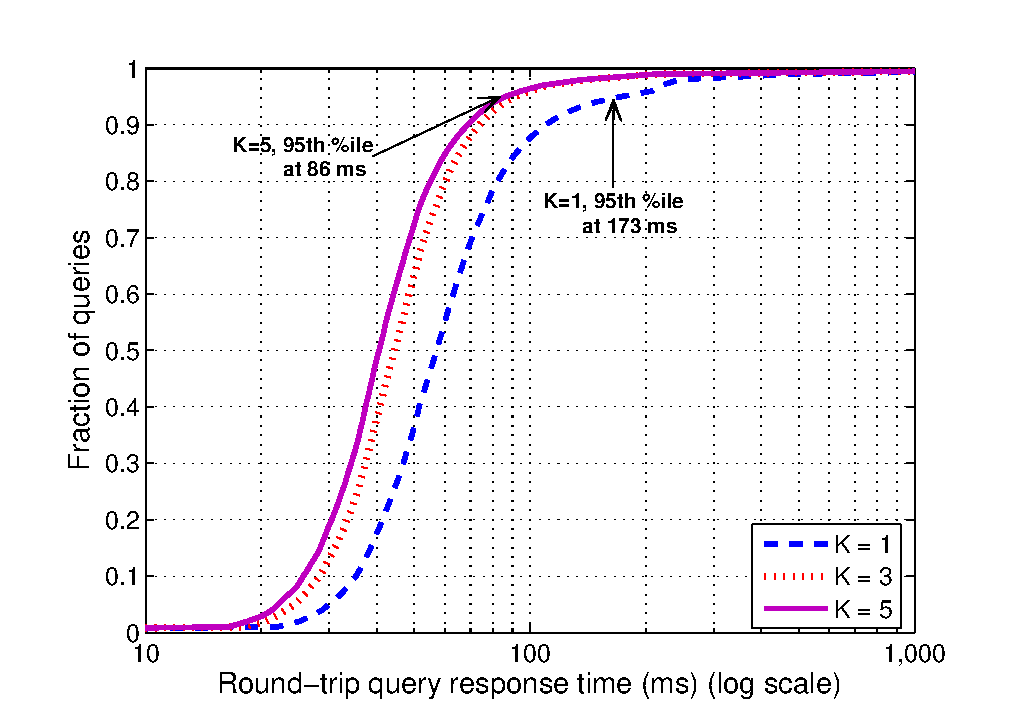
\includegraphics[width=0.4\textwidth]{figures/queryLatency}
	\caption{Round trip query response times}
	\label{fig:queryLatency}
	\vspace{-0.15in}
	\end{figure}
\end{center}

\vspace{-0.3in}

\subsubsection{Results}
We present two sets of results that characterize the query response time and the load distribution of our scheme respectively.

\paragraph{Query Response Time} We evaluate the query response time for DMap
by inserting $10^5$ GUIDs and generating $10^6$ queries according to the popularity model. By repeated trials with increasing number of GUIDs/queries, we
verified that the response times converged after reaching the above configuration and larger numbers are not necessary. When we store a mapping at multiple locations, i.e., $K>1$, in the results below, we assume that the querying node has sufficient information to choose the location with the lowest response time. We note that in today's Internet, this information is only partially available, but at the least, each AS has hop count information for reaching
all other ASs through the routing protocol. Using least
hop count instead of lowest response time leads to similar results
albeit with marginally increased latencies. We would also emphasize that many techniques are being proposed to better estimate the response times~\cite{Godfrey2009}.

 %(for example, median latency changes from
%40ms to 50ms for the $K=5$ curve in Figure~\ref{fig:queryLatency})


%{\bf Thu: need to
%work in a few words about what happens if we use hop counts
%  instead.}

Figure~\ref{fig:queryLatency} plots the
cumulative distribution function (CDF) of the round trip query
response times with varying $K$ values. We make two observations. First, with $K=5$, 95\% of the queries complete within 86ms. This is well within the range needed for voice
call handoffs~\cite{3gpp}. Indeed, given that many WiFi and IP handoff protocols are often on the order of 0.5-1 second~\cite{vassiliou_2009,Mishra:2003:EAI:956981.956990},
DMap updates would not introduce an undue additional burden. Second, storing each GUID mapping in multiple locations can significantly reduce query response
times, as it allows a querying node to choose the replica that is
``closest'' to itself, thus addressing the locality of the requests. The effect of increasing $K$ can be clearly seen with the leftward shift of the CDF curve as we increase the value
of $K$. In particular, the mean, median and $95^{th}$ percentile query
latencies of $K = 1$ and $K = 5$ cases are tabulated in
Table~\ref{table:latency}, which shows a marked decrease in the tail of the response time distribution.

However, even the curve for $K=5$ has a relatively long tail.  This long tail arises from a few queries originating from those ASs with unusually long intra-AS response times, according to the DIMES dataset. For example, the 18 queries with the longest response times all originated from AS 23951, a small AS registered in Indonesia with a one-way latency of more than 2.3 seconds on each of its outgoing links.
\begin{table}[b]
\vspace{-0.1in}
\centering
\begin{tabular}{|c|c|c|c|}
\hline
\multicolumn{1}{|c|}{{\bf {\em K}}} & \multicolumn{3}{|c|}{{\bf Round Trip
    Query Response Time (ms)}}\\
\cline{2-4}
 & {\bf Mean} & {\bf Median} & {\bf 95th percentile}\\
\hline
1 & 74.5 & 57.1 & 172.8\\
\hline
5 & 49.1 & 40.5 & 86.1\\
\hline
\end{tabular}
\caption{Query Response Time Statistics for $K $ = 1, 5}
\label{table:latency}
\end{table}

\begin{center}
\begin{figure}[t]
\vspace{-0.2in}
\centering
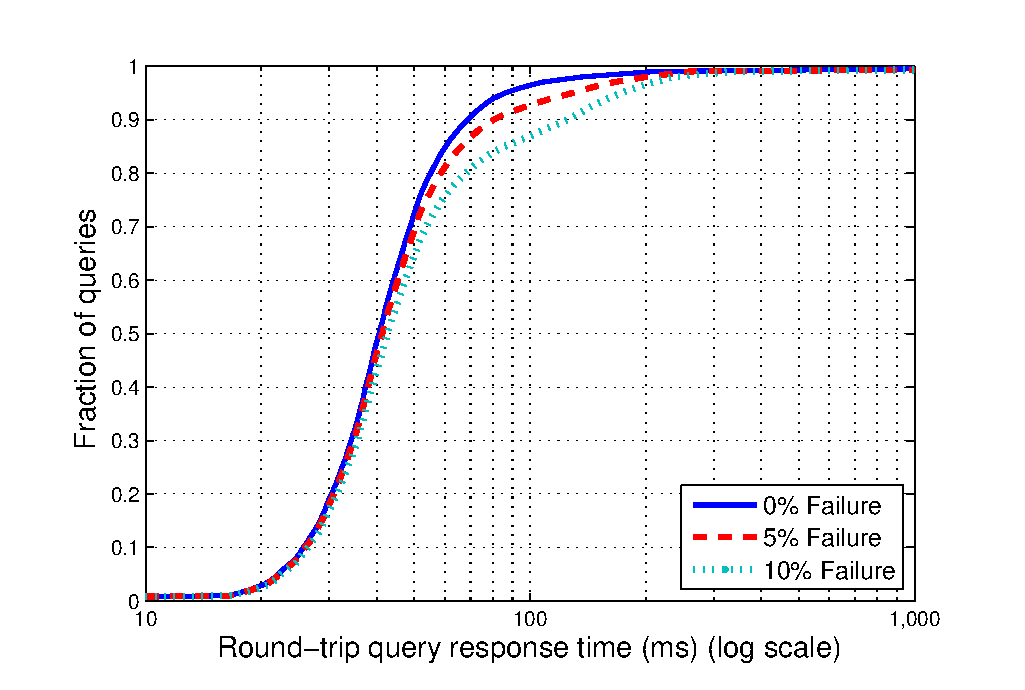
\includegraphics[width=0.4\textwidth]{figures/queryLatencyVsChurn}
\caption{Effect of BGP Churn on query response times.}
\label{fig:queryLatency-BGP-churn}
\vspace{-0.2in}
\end{figure}
\end{center}

\vspace{-0.3in}

\paragraph{Impact of BGP Churn}  %{\bf (Thu: this is very rough.  It
  %would be nice if Rich or Yanyong or someone who understands BGP
 % better than I can help improve this paragraph a little bit.}
The above study assumes that the BGP table at the query origin exactly
reflects the current state of the Internet. However, BGP tables at
different places in the Internet can be inconsistent because of new prefix announcements or prefix withdrawals. This inconsistency may have an adverse impact on the overall query response times as the query may reach an AS which does not host the requested mapping. In this situation, the AS will then reply with a ``GUID missing'' message, and the querying node will have to contact another replica.  %{\bf Thu: Can this
%  lead to another failure?}
Thus, a query may require multiple round-trips to different ASs for each resolution.
We note that the probability of two churns occurring at the same time for the same GUID is negligible.
  %Since our hashing scheme only depends on the information on
%the source AS for IP prefixes, we only need to consider BGP updates
%that result in origin AS changes for any IP prefix.
%
%In~\cite{qiu-2006}, the authors observe that ``origin changes account
%for less than 2\% of the BGP update traffic with more than 90\% of the
%prefixes being consistently originated by the same AS for an entire
%year. For those prefixes involved in origin changes, approximately 57\% have only one change across the year, implying that these changes are indeed permanent.'' In~\cite{mahajan-NANOG23}, Mahajan et al. observe that ``more than 2\% of the prefixes experience an origin change during the day.''
Here, we conduct a set of experiments to quantify the impact of this inconsistency caused by BGP churn. In the experiments, we vary the percentage of prefixes that are newly announced or withdrawn from 0 to 10\%. Figure~\ref{fig:queryLatency-BGP-churn} plots the CDF of the query
response times for $K=5$ and 0\% to 10\% lookup failures.  A 5\%
failure rate, which already seems pessimistic according
to~\cite{qiu-2006,mahajan-NANOG23}, shifts the median and 95th
percentile from 40.5ms and 86.1ms to 41.3ms and 129.1ms,
respectively.  %{\bf Thu: Akash, Tam, in the powerpoint, you have
 % numbers of 20\% failure rate.  But, I think that this is too
 % pessimistic.  I prefer using the 5\% numbers unless you think that
 % this is wrong.} \textbf{Akash: Sure, I entered the values}

\vspace{0.1in} \paragraph{Storage Distribution}
We next study the distribution of GUID$\rightarrow$NA mappings amongst ASs to evaluate
DMap's ability to spread the storage load proportional to the size of
the ASs. We measure storage load using the {\em Normalized Load
  Ratio} (NLR) at each AS, which is defined as the ratio of the
percentage of GUIDs assigned to an AS divided by the percentage of IP
addresses advertised by that AS. For example if an AS announces a $/8$
prefix, corresponding to 0.39\% of the 32 bit IP space and is assigned
20,000 out of a total of 1 Million GUIDs, i.e., 2\% of GUIDs, then its
normalized load would be 2/0.39 $\simeq$ 5. Ideally, each AS's NLR
would be 1.

Figure~\ref{fig:loadDistr} plots the CDF of the NLR when we inserted
from $10^5$ to $10^7$ GUIDs, with $K=5$.
%(In this experiment, $K>1$ simply equals inserting more GUIDs so we only discuss results for $K=1$.)
We observe that for $10^7$ GUIDs, %88\% of the ASs had NLRs between
%0.5 and 1.5 {\bf Can change the 0.5 to 1.5 a little bit to get a
%  ``nicer'' percentage if desired}. \textbf{Akash: Maybe,
93\% of the ASes had NLRs between 0.4 and 1.6. Further, we observe that as the
number of GUIDs increases from $10^5$ to $10^7$, the CDF becomes much
sharper around NLR equal to 1 (with a shorter tail). This suggests that DMap can distribute the storage load better when the system scales.
%distribution of
%storage load improves with the number of GUIDs in the system.
These results show that DMap does a %extremely
very good job of spreading out the
storage load proportional to the percentage of the IP space that an AS
claims.

Interestingly, the median NLR value is 1.16. The fact that the median NLR value is greater than 1 is expected since in addition to its fair share of GUIDs, many ASs are also allocated a portion of the GUIDs that has hashed values after M retries falling in the IP holes as described in Section~\ref{subsec:ip_hole}.

%we have also studied the tail of the CDF for $10^7$ GUIDs in
%Figure~\ref{fig:loadDistr}. There were only 16 ASs with NLR greater
%than 3. None of these ASs received additional load because of IP
%holes. %{\bf Thu: Akash, Tam, please check this if you can. If you can
  %only check a subset, let me know.} \textbf{Akash: Checked all; none of the 16
  %announces addresses which are adjacent to a hole.} All of these are small ASes,
%i.e., advertising 256--2304 addresses, that received several extra
%GUIDs.  We believe that such slight overloading is not a problem, and
%will further reduce as the number of GUIDs increase.
\iffalse
	\begin{table}[b]
	\centering
	\begin{tabular}{|c|c|c|c|}
	\hline
	\% Local & Mean & Median & 95th Percentile\\
	Queries & Response Time & Response Time & Response Time\\
	\hline
	0 & 49.1 & 40.5 & 86.1\\
	\hline
	10 & 45.9 & 38.6 & 84.1\\
	\hline
	20 & 43.2 & 36.8 & 82.2\\
	\hline
	30 & 40.4 & 34.6 & 80.2\\
	\hline
	\end{tabular}
	\caption{Round trip response time (ms) for varying spatial locality ($K =5$)}
	\label{table:locality}
	\end{table}
\fi
%Modeling host mobility in the Internet has been the focus of a large number of studies, though most models aim to characterize specific wireless environments, for example, cellular networks~\cite{Hyytia-07}, vehicular networks~\cite{Harri-06} and ad-hoc networks~\cite{Lin-04}. Since our focus is not on modeling the movement of hosts but to capture the GUID-to-NA mapping update they might produce, we abstract out a simple discrete model for the number of mapping updates for each GUID. In this model, GUIDs are classified into four broad classes: fast mobility, medium mobility, low mobility and static. Inter-update times in each of the three mobile classes are distributed exponentially with a different mean value per class. The proportion of fixed and mobile hosts is kept as a parameter $\beta$, while the probability of a mobile host belonging to each of the three mobile classes being kept equal. In order to include the reality of most popular hosts being static, we include a parametric threshold $\tau$, which defines the popularity level above which all hosts are static. Figures ? and ? shows the popularity and mobility models used in our simulation.

%It then produces a inter-domain routing table for all ASs in the network. We consider that each AS has one participating BGP router.
\iffalse
	\begin{center}
	\begin{figure}[t]
	%\vspace{-0.2in}
	\centering
	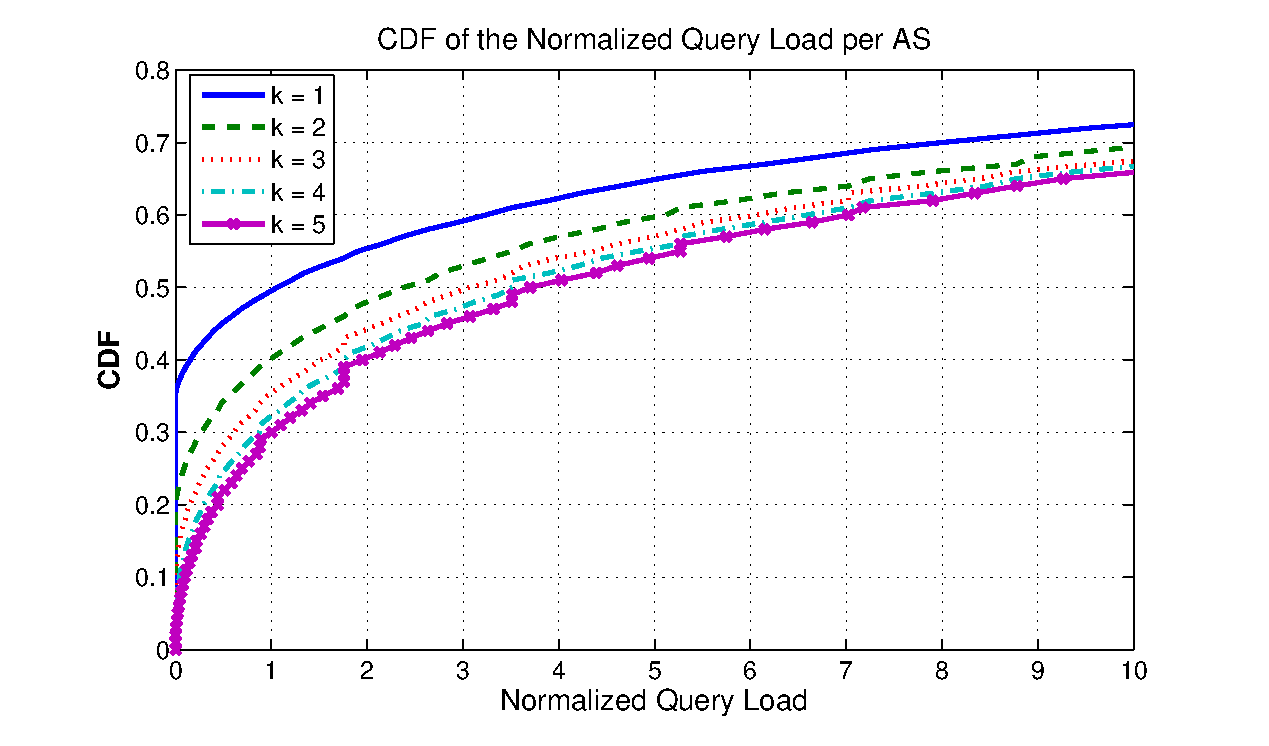
\includegraphics[width=0.5\textwidth]{figures/queryLoadVsK1}
	\caption{Empirical CDF of the Normalized Query Load}
	\label{fig:queryLatency}
	%\vspace{-0.2in}
	\end{figure}
	\end{center}
	
	\begin{center}
	\begin{figure}[t]
	%\vspace{-0.2in}
	\centering
	\includegraphics[width=0.5\textwidth]{figures/storageLoadK-5}
	\caption{Empirical CDF of the Normalized Storage Load}
	\label{fig:queryLatency}
	%\vspace{-0.2in}
	\end{figure}
	\end{center}
	
	\begin{center}
	\begin{figure}[t]
	%\vspace{-0.2in}
	\centering
	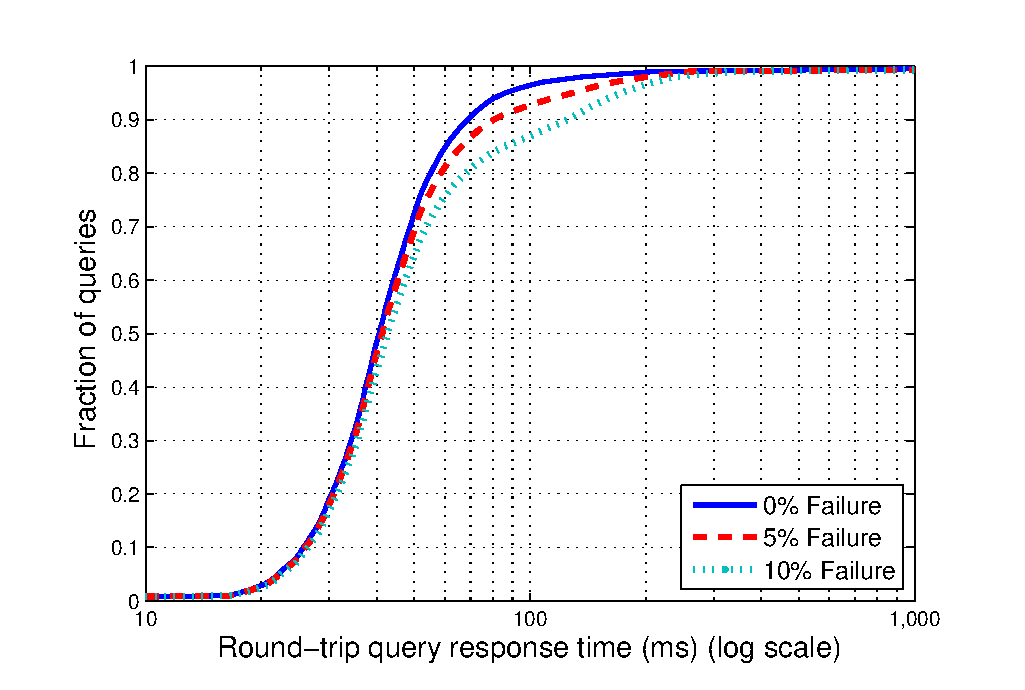
\includegraphics[width=0.5\textwidth]{figures/queryLatencyVsChurn}
	\caption{Effect of BGP Churn on query latency}
	\label{fig:queryLatency}
	%\vspace{-0.2in}
	\end{figure}
	\end{center}
\fi
%\subsection{Future Internet model}

%TBA

%Jun's estimation goes here


%This section present our large scale simulation implementation.

%Our simulation takes description of the network topology at layer-3 from netDimes \cite{} including 90 thousands single-hop AS-to-AS connection, from which we build the connectivity graph between ASes. We derives from 9 Millions  end-to-end traces from netDimes to have an estimation of intra-AS latency for every AS. Let $L_{AS1}$ and $L_{AS2}$ are intra AS latency of AS1 and AS2 accordingly.  If there is a connectivity from AS1 to AS2, the latency for every single-hop AS-to-AS connection is compute as follow.

%We takes a list of IP prefixes from \cite{}, a Japanese BGP border gateway. it produces a inter-domain routing table for all routers in the network. That route selection process computes the shortest path according to  from the provided topology. One might argues that the route selection should follow BGP which also takes ASes' policies into account. However,  for simplicity, all policies should be reflected on the provided topology in our model, e.g. if an AS prefers one path over another, that preference should be represented in path's cost. Note that edges are directional.

%Once the topology is loaded, and the inter-domain routes have been computed, the Actuator starts processing events in global queue in sequential order. The global queue guarantees that the orders of events on each run are the same and will lead to the same outcome. That is in contrast with traditional discrete event where outcome depends on the seed of the pseudo random number generator. There are several types of events, including  GUID insert, GUID update, GUID lookup and BGP table update.

%For each insertion event extracted from the global even queue, Actuator applies k hash function on to that GUID, may rehash up to m times to get the hashed value felt into announced IP address, called IPx. For each IPx, Actuator lookup on AS prefix table to find the corresponding AS and destination IP address of BGP speaker's of that AS. It then get the list of  ASes that the request must be directed through in order to be delivered to that destination AS. For each AS on the path, Actuator updates the message counter of that AS, adjust the time stamp on that AS, and increase the time stamp for that request based on the latency of the passed through link. For timestamp adjustment on particular AS, Actuator assign the greater timestamp among <AS time stamp, message time stamp>  as the new time stamp for that AS. The message is forwarded on a AS-by-AS basis until it reaches its final destination. Upon delivered to the destination, destination AS update its GUID list with the new one, followed by GUID's time stamp.

%The actuator continues the simulation by popping the first event from the global queue, simulating the behavior at each router along the path. If the event is GIUD lookup or GIUP date, the steps tobe executed by the actuator are very much similar to that with aforementioned GUID insert.  If the event is BGP table update, the actuator takes the diff operation to compare the old table with the new one. It then identifies ASes that got affected from the change�


%We evaluate the DMap architecture using three different views of the structure of the Internet:

%(TBA:Change the three names)

%\begin{enumerate}
%\item Present day Internet: As a first step, we evaluate the performance of DMap over the Internet as it is today using measurement based model comprised of $\sim$17,000 ASs and $\sim$190,000 Points of Presence (PoPs). The connectivity graph between PoPs, link latencies and path prediction is derived from the iPlane project~\cite{IplaneNano09}, which provides a structural view of the Internet using measurements from distributed vantage points in the network.

%\item Removing the effects of path inefficiencies: To isolate the effects of path inefficiencies in the Internet from the irreducible path characteristics, we re-evaluate the performance numbers assuming a shortest path routing between ASs. The results show that a major portion of network delays are an artifact of path inefficiencies in the Internet which can be alleviated by routing improvements in the future Internet.
%
%\item Future Internet model: Finally, we define a simplistic, but pragmatic model of the future Internet topology and discuss the deployment and performance of the proposed DMap architecture in this context.
%
%\end{enumerate}
%%In this section, we present results from a large-scale event-based simulation study aimed at characterizing the performance of DMap. Our evaluation focuses on the following performance measures:

%%\subsection{Present day Internet}
%%
%In this section, we present results from a large-scale measurement driven, event-based simulation study aimed at characterizing the performance of DMap. Our evaluation focuses on the following performance measures:
%
%\begin{itemize}
%\item Query and Update Latency (Fig. ? \& Fig. ?)
%\item Storage Load Distribution ( )
%\item Query and Update Load Distribution ( )
%\item Probability of Retrieving Stale Mappings ( )
%\end{itemize}
%
%
%\subsubsection{Simulation setup}
%\label{subsec:evaluation_setup}
%
%%\subsubsection{Event-based Simulator Architecture}
%
%The discrete-event simulator consists of a measurement driven Internet topology model with $\sim$17,000 ASs encompassing $\sim$190,000 Points of Presence (PoPs). The connectivity graph between PoPs, link latencies and path prediction is derived from the iPlane project~\cite{IplaneNano09}, which provides a structural view of the Internet using measurements from distributed vantage points in the network. Two types of events: GUID updates and GUID queries are generated according to parametric popularity and mobility models, as described in Sec. ?. Each event is associated with a 3-tuple of \emph{ $<$ GUID $|$ Timestamp $|$ Source of query/update$>$}. The event list is pre-generated and organized into a global queue which guarantees that the order of events on each run are the same and will lead to the same outcome. The event controller processes events in the global queue in sequential order following the sequence of operations outlined in Section~\ref{sec:design} to process each kind of event. Data gathering is done per-event for end-to-end latency, staleness and per-AS for number of GUIDs stored, queries and updates received\footnote{The source code for our simulation is made available at \cite{sourceCode_NRS}}.

\begin{center}
\begin{figure}[t] 
\vspace{-0.2in}
\centering
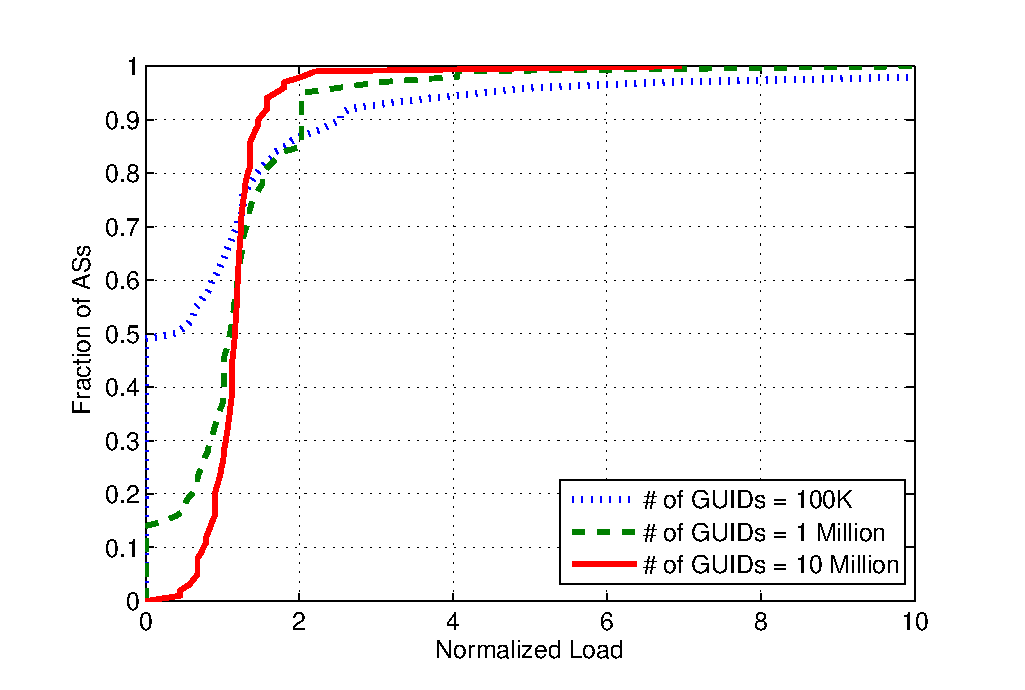
\includegraphics[width=0.4\textwidth]{figures/loadDistr}
\caption{Normalized Load Ratio per AS}
\label{fig:loadDistr}
\vspace{-0.2in}
\end{figure}
\end{center}
\vspace{-0.2in}




%%% Local Variables:
%%% mode: latex
%%% TeX-master: "paper"
%%% End:
